


\section{Passive Attack and Active Attack}

The CPA Security can defend passive attack, however, it cannot defend active attack. In active attack, the attacker can not only get the plaintext, it can also get the ciphertext.

For example in Figure \ref{fig: 05 Example of Active Attack to MAC}. If the attacker get to know the ciphertext and message of the two message. It can easily generate a new (m,c,t) pair that is available. It can be done by just use $I V^{\prime}=I V \oplus(\ldots 80 \ldots) \oplus(\ldots . .25 \ldots)$.

\begin{figure}[h]
    \centering
    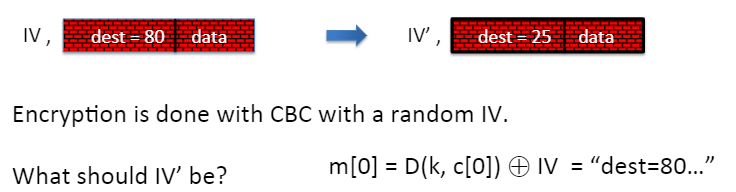
\includegraphics[width=0.5\textwidth]{Stanford_Crypto_1/fig/05_Authentication/An active attack to MAC.png}
    \caption{Example of Active Attack to MAC}
    \label{fig: 05 Example of Active Attack to MAC}
\end{figure}

So we have the conclusion that "CPA security cannot guarantee secret under active attacks". We should choose methods from:

\begin{enumerate}
    \item If message needs integrity but no confidentiality, use a MAC
    \item If message needs both integrity and confidentiality, use authenticated encryption modes
\end{enumerate}

\section{Chosen Ciphertext Attacks}

Adversary's power: both CPA and CCA
\begin{itemize}
    \item Can obtain the encryption of arbitrary message of his choice
    \item Can decrypt any ciphertext of his choice, other than challenge
\end{itemize}

The experiment about CCA is shown in Figure \ref{fig: 05 CCA Experiment}

\begin{figure}[h]
    \centering
    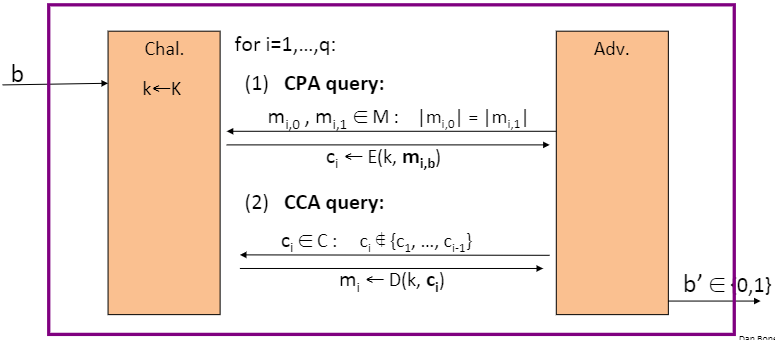
\includegraphics[width=0.5\textwidth]{Stanford_Crypto_1/fig/05_Authentication/CCA Experiment.png}
    \caption{CCA Experiment}
    \label{fig: 05 CCA Experiment}
\end{figure}

So we can define the security under CCA:

\begin{definition} [CCA Security]
    $\mathrm{E}$ is CCA secure if for all "efficient" A:
    $$
    \operatorname{Adv}_{C C A}[A, E]=|\operatorname{Pr}[\operatorname{EXP}(0)=1]-\operatorname{Pr}[\operatorname{EXP}(1)=1]| \text { is "negligible." }
    $$
    
\end{definition}

\section{Ciphetext Integrity}

The experiment for Ciphertext Integrity is shown in Figure \ref{fig: 05 Ciphertext Integrity}.

\begin{figure}[h]
    \centering
    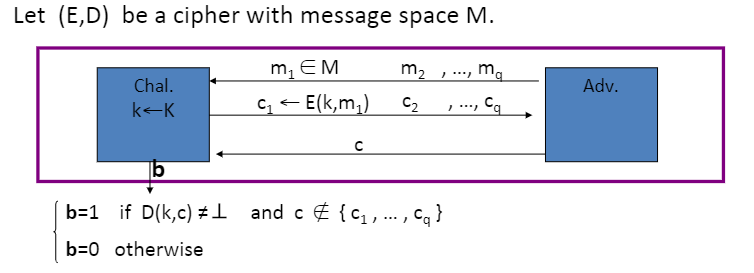
\includegraphics[width=0.5\textwidth]{Stanford_Crypto_1/fig/05_Authentication/Ciphertext Integrity.png}
    \caption{Ciphertext Integrity}
    \label{fig: 05 Ciphertext Integrity}
\end{figure}

Then we can define the Ciphertext Security:

\begin{definition} [Ciphertext Security] Ciphertext Security
    
    (E,D) has $\underline{\text { ciphertext integrity }}$ if for all "efficient" $A$ :
    $\operatorname{Adv}_{\mathrm{CI}}[A, E]=\operatorname{Pr}[$ Chal. outputs 1] $\quad$ is "negligible."
    
\end{definition}


\section{Authenticated Encryption}

\subsection{Conceptions}

\begin{definition}[Authenticated Encryption]  Authenticated Encryption
    
    An authenticated encryption system $(E, D)$ is a cipher where
    As usual:
    $\mathrm{E}: \mathrm{K} \times \mathrm{M} \times \mathrm{N} \rightarrow \mathrm{C}$
    but
    D: $K \times C \times N \rightarrow M \cup\{\perp\} \textbf{(which means the ciphertext is rejected)}$

\end{definition}

And we want the system provide:
\begin{itemize}
    \item Sem.Sec under a CPA attack
    \item Ciphertext integrity: attacker cannot create new ciphertexts that decrypt properly.
\end{itemize}


\begin{definition} [Authenticated Encryption Cipher] Authenticated Encryption Cipher:

    Cipher (E,D) provides authenticated encryption (AE) if it is:
    \begin{itemize}
        \item semantically secure under CPA, and
        \item has ciphertext integrity
    \end{itemize}
    
\end{definition}

A authenticated encryption cipher imply two things:
\begin{enumerate}
    \item Attacker cannot fool Bob into thinkging a message was sent from Alice: if $D(k, c) \neq \perp$ Bob knows message is from someone who knows $k$ (but message could be a replay)
    \item security against chosen ciphertext attack
\end{enumerate}


\subsection{Security Analysis}

\begin{theorem} [Authenticated Encryption and CCA Security] Authenticated Encryption and CCA Security

    Let $(E, D)$ be a cipher that provides $A E$.
    Then (E,D) is CCA secure!
    In particular, for any q-query eff. A there exist eff. B $_{1}, B_{2}$ s.t.
    $A d v_{C C A}[A, E] \leq 2 q \cdot A d v_{C C}\left[B_{1}, E\right]+A d v_{C P A}\left[B_{2}, E\right]$
        
\end{theorem}


\subsection{Constructions from Ciphers and MACs}

\subsubsection{MAC-then-Encrypt}

One example (SSL) of MAC-then-Encrypt  is shown in Figure \ref{fig: 05 MAC-then-Encrypt}. 


\begin{figure}[h]
    \centering
    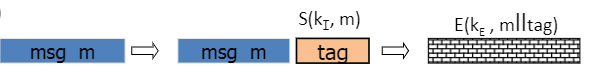
\includegraphics[width=0.5\textwidth]{Stanford_Crypto_1/fig/05_Authentication/M then E.png}
    \caption{MAC-then-Encrypt}
    \label{fig: 05 MAC-then-Encrypt}
\end{figure}


\subsubsection{Encrypt-then-MAC}

One example (IPsec) of Encrypt-then-MAC  is shown in Figure \ref{fig: 05 Encrypt-then-MAC}. 


\begin{figure}[h]
    \centering
    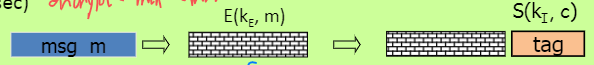
\includegraphics[width=0.5\textwidth]{Stanford_Crypto_1/fig/05_Authentication/E then M.png}
    \caption{Encrypt-then-MAC}
    \label{fig: 05 Encrypt-then-MAC}
\end{figure}


\subsubsection{Encrypt-and-MAC}

One example (SSH) of MAC-and-Encrypt  is shown in Figure \ref{fig: 05 Encrypt-and-MAC}.


\begin{figure}[h]
    \centering
    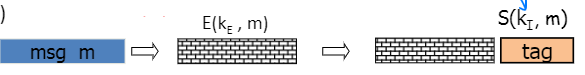
\includegraphics[width=0.5\textwidth]{Stanford_Crypto_1/fig/05_Authentication/E and M.png}
    \caption{Encrypt-and-MAC}
    \label{fig: 05 Encrypt-and-MAC}
\end{figure}


\subsubsection{Some Standard}

GCM, CCM, EAX.

All support AEAD (auth.enc.with associated data). All are nonce-based.

\subsection{Security Analysis}

Let (E,D) be CPA secure cipher and (S,V) secure MAC, then:

\begin{enumerate}
    \item Encrypt-then-MAC always provides A.E.
    \item MAC-then-Encrypt may be insecure against CCA attacks. However, wehn (E,D) is rand-CTR mode or rand-CBC, then it will be A.E.
\end{enumerate}

\subsection{Direct Construction from PRP: OCB}

The OCB frame work is shown in Figure \ref{fig: 05 OCB}.


\begin{figure}[h]
    \centering
    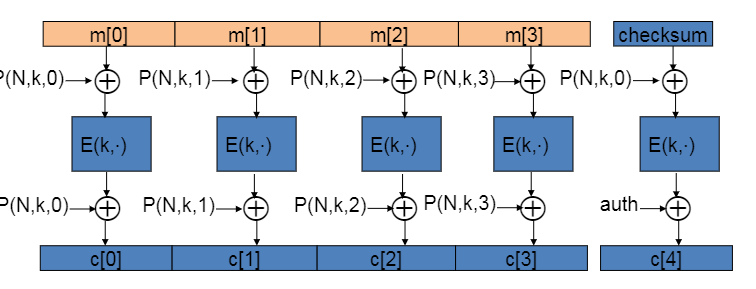
\includegraphics[width=0.5\textwidth]{Stanford_Crypto_1/fig/05_Authentication/OCB.png}
    \caption{OCB}
    \label{fig: 05 OCB}
\end{figure}


\subsection{CBC padding attacks}

Some lessons about CBC padding attacks:
\begin{itemize}
    \item Encrypt-then-MAC would completely avoid this problem
    \item MAC-then-CBC provides A.E., but padding oracle destroys it
\end{itemize}

\section{Summary}

Starting from the property of active attacker, we explained why the MAC cannot defend active attacker with an example. Then based on the fact that an active attacker can always see the ciphertext, we define the definition of ciphertext integrity and CCA Security.

Then we propose that Authenticated Encryption, that should be able to meet integrity and authenticated and be Sem. Sec under CCA. Then we introduce 3 ways to build an AE from MAC: E then M, M then E, M and E. And the fact is E then M always meet AE. Besides, we also mentioned one method to build an AE from PRP, the OCB method.